\documentclass{beamer}

\usepackage{amsmath,amssymb,amsthm}
\usepackage{algorithm,algorithmic}
\usepackage{txfonts}
\usepackage{subfigure}
\usepackage{pgf,tikz}
\usepackage{multirow}
\usepackage{subfigure}
\usepackage{epstopdf}
\usepackage{float}
\usepackage{ulem}
\usetikzlibrary{shapes,arrows,automata}
\setbeamercovered{transparent}

\newtheorem{thm2}{Theorem}[section]

\newcommand{\Pow}{\mathbf{P}}
\newcommand{\tabincell}[2]{\begin{tabular}{@{}#1@{}}#2\end{tabular}}

%\usetheme{Warsaw,Antibes,Madrid,JuanLesPins,bars}
\usetheme{CambridgeUS}
%\usetheme{Hannover,Singapore}
\begin{document}


    \title[SemEval2016 STS-Task]{Leveraging Word Embedding from Macro and Micro View to Boost Performance for Semantic Textual Similarity}
    \author[TIAN JunFeng]{}
    \institute[ECNU]{}
    \date{\today}

    \frame{\titlepage}

\section{Outline}
\frame{
\frametitle{Outline}
\begin{itemize}
\item Task Definition
\item Our Systems
    \begin{itemize}
        \item Preprocess
        \item Traditional NLP Feature Engineering
        \item Word Embedding Feature Engineering
    \end{itemize}
\item Experiments
\item Results
\item Conclusion
\end{itemize}
}
\section{Task Definition}

% Task Definition
% Example
\frame{
\frametitle{Task Definition}
\begin{definition}[Semantic Textual Similarity]
\textbf{Input}: \qquad given two sentences \\
\textbf{Output}: \quad similarity score({\color{red}[0,5]}) \\
\textbf{Gold Standard}: human judgements \\
\textbf{Evaluation}: Pearson correlation \\
\end{definition}

\begin{block}{Example}
$   
    \left\{ \begin{array}{ll}
    \textrm{ The bird is bathing in the sink.}\\
    \textrm{ Birdie is washing itself in the water basin.} \\
    \end{array} \color{red}{ \text{\quad \ (sys: ? / gs: 5.0)}} \right.
$
\vspace{0.5cm}

$   \left\{ \begin{array}{ll}
    \textrm{ The woman is playing the violin.}\\
    \textrm{ The young lady enjoys listening to the guitar.}\\
    \end{array} \color{red}{ \text{(sys: ? / gs: 1.0)}} \right.
$
\end{block}
}

% Motivation

\section{Our Systems}

\frame{
\frametitle{Our Systems}
{\color{blue}Traditional NLP Feature Engineering}
\begin{enumerate}
\item String-Based Similarity
\item Machine Translation Similarity
\item Corpus-based Features
\item Alignment Measures
\end{enumerate}
\vspace{0.5cm}
{\color{blue}Word Embedding Feature Engineering}
\begin{enumerate}
\item Word Centroid Distance
\item Word Mover's Distance
\end{enumerate}
}


\subsection{Preprocess}

\frame{
\frametitle{Preprocess}
\begin{enumerate}
\item To Formal Writing (Search and Replace)\\
            e.g., doesn't $\rightarrow$ does not
\item Lemmatize (NLTK and Stanford CoreNLP)\\
             e.g., was  $\rightarrow$ be
\item Parse (Stanford CoreNLP)
    \begin{itemize}
        \item[POS tag]
            \begin{figure}[h]
            {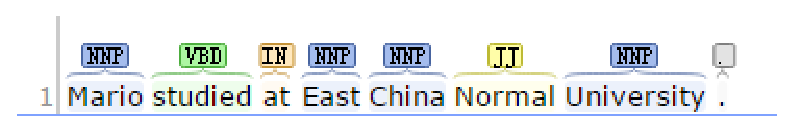
\includegraphics[width=0.45\columnwidth]{figs/pos.eps}}
            \end{figure}
        \item[NER tag]
            \begin{figure}[h]
            {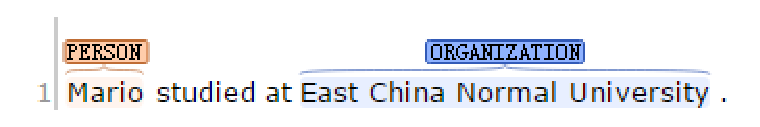
\includegraphics[width=0.45\columnwidth]{figs/ner.eps}}
            \end{figure}
    \end{itemize}
\end{enumerate}
}

\subsection{Traditional NLP Feature Engineering}

\frame{
\frametitle{Traditional NLP Feature Engineering}
\begin{enumerate}
\item String-Based Similarity
\item Machine Translation Similarity
\item Corpus-based Features
\item Alignment Measures
\end{enumerate}
}

\frame{
\frametitle{String-Based Similarity}
\begin{itemize}
\item {\bf Length Features (len):}
        $$|A|, |B|, |A-B|, |B-A|, |A \cup B|, |A \cap B|, \frac{|A-B|}{|B|}, \frac{|B-A|}{|A|}$$

    %Since two sentences with similar syntax structure convey similar meaning, we estimate the similarities of syntax structure.
\item {\bf Syntactic Features (pos):}
        $$|A_{pos}|, |B_{pos}|, |A_{pos}-B_{pos}|, |B_{pos}-A_{pos}|$$
        $$ |A_{pos} \cup B_{pos}|, |A_{pos} \cap B_{pos}|, \frac{|A_{pos}-B_{pos}|}{|B_{pos}|}, \frac{|B_{pos}-A_{pos}|}{|A_{pos}|}$$

\item {\bf Longest Common Sequence (lcs):}
        $$\frac{|lcs(A, B)|}{min(|A|, |B|)}$$
    %In consideration of the different length of sentence pairs, we normalize the maximum length of the common subsequence of two sentences with the length of the shorter one.
\end{itemize}
}

\frame{
\frametitle{String-Based Similarity}
\begin{itemize}
\item {\bf Ngrams Overlap Features (ngram):}  \\
            \begin{enumerate}
                \item word level (original and lemmatized) / character level. \\
                \item $n = \{1, 2, 3\}$ are used for the word level. \\
                \item $n = \{2, 3, 4\}$ are used for the character level. \\
            \end{enumerate}
\vspace{0.5cm}
\item {\bf Named Entities Features (ner): } \\
        \vspace{0.2cm}
         location, organization, data, money, person, time, percent
\end{itemize}
}

\frame{
\frametitle{Machine Translation Similarity}
\textbf{Machine Translation Similarity}
\begin{block}{}
1. Viewed as one input and one output of a MT system. \\
\vspace{0.3cm}
2. MT measures (i.e., { WER, TER, PER, NIST, ROUGE-L, GTM-1})\\
\vspace{0.3cm}
3. Two strategies (i.e., { average } and { concatenate})\\
\end{block}
}


\frame{
\frametitle{Corpus-based Features}
\begin{itemize}
\item {\bf WordNet Rank Features (wordnet):}
    \begin{enumerate}
        \item normalized ranking (sentence) vector.
        \item sentence vector distance: cosine, manhattan, Euclidean, Jaccard.
    \end{enumerate}
\vspace{0.5cm}

\item {\bf Vector Space Sentence Similarity (lsa):}
    \begin{enumerate}
        \item  Latent Semantic Analysis(LSA)
        \item  New York Times Annotated Corpus(NYT) / Wikipedia
        \item  convert to sentence level: sum up / use idf to weigh each word vector.
    \end{enumerate}
\end{itemize}
}

\frame{
\frametitle{Alignment Measures}
	
$$   \left\{ \begin{array}{ll}
    \text{\em 12 {\color{blue}killed in} bus  {\color{blue}accident in} {\color{blue}Pakistan.}}\\
    \text{\em 10 {\color{red}killed in} road {\color{red}accident in} NW {\color{red}Pakistan.}}\\
    \end{array}  \color{black}{ \text{\quad \ (sys: (2/3)*5 / gs: 3.2)}} \right.
$$

\begin{itemize}
\item \textbf{Global Alignment Features:} \\
$$ sim(S_1, S_2) =  \frac{n_a(S_1) + n_a(S_2)}{n(S_1)+n(S_2)} $$

\item \textbf{POS-Specific Alignment Features:} \\
\vspace{0.3cm}
{calculate the aligned words proportion specifically \\ according to POS tag(i.e., noun, verb, adjective, adverb).}\\
%Taking weight of POS tag of aligned words into consideration, score of aligned {\em noun} word pair is surely higher than the {\em adjective}. Using this property, we propose the specific alignment feature, to
\end{itemize}
}

\subsection{Word Embedding Feature Engineering}

\frame{
{Word Embedding Feature Engineering}

\begin{enumerate}
\item<1> Word Centroid Distance
\item<2> Word Mover's Distance
\end{enumerate}
\only<1> {
\begin{figure}[b]
\small
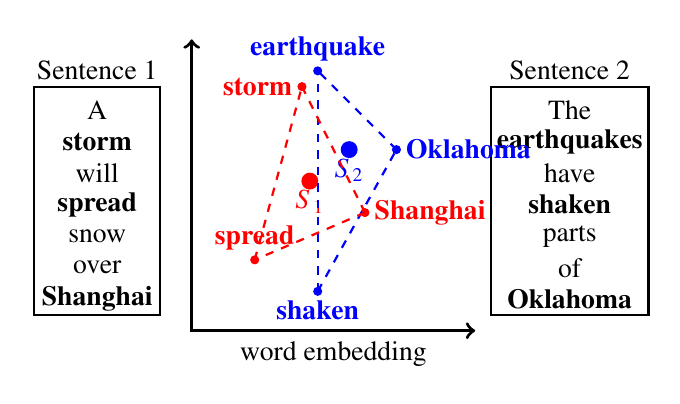
\begin{tikzpicture}
\draw [thick] (0.2, 0.5) rectangle (1.8, 3.4);
\draw [very thick, <->] (2.2, 4.0) -- (2.2, 0.3) -- (5.8, 0.3);
\draw [thick] (6.0, 0.5) rectangle (8.0, 3.4);

\node at (4.0, 0.0) {word embedding};

\node at (1.0, 3.6) {Sentence 1};
\node at (1.0, 3.1) {A};
\node at (1.0, 2.7) {\bf storm};
\node at (1.0, 2.3) {will};
\node at (1.0, 1.9) {\bf spread};
\node at (1.0, 1.5) {snow};
\node at (1.0, 1.1) {over};
\node at (1.0, 0.7) {\bf Shanghai};

\node at (7.0, 3.6) {Sentence 2};
\node at (7.0, 3.1) {The};
\node at (7.0, 2.7) {\bf earthquakes};
\node at (7.0, 2.3) {have};
\node at (7.0, 1.9) {\bf shaken};
\node at (7.0, 1.5) {parts};
\node at (7.0, 1.1) {of};
\node at (7.0, 0.7) {\bf Oklahoma};

\draw [fill, red] (3.6, 3.4) circle [radius=0.05];
\node [left, red] at (3.6, 3.4) {\bf storm};

\draw [fill, blue] (3.8, 3.6) circle [radius=0.05];
\node [above, blue] at (3.8, 3.6) {\bf earthquake};

\draw [fill, red] (3.0, 1.2) circle [radius=0.05];
\node [above, red] at (3.0, 1.2) {\bf spread};

\draw [fill, blue] (3.8, 0.8) circle [radius=0.05];
\node [below, blue] at (3.8, 0.8) {\bf shaken};

\draw [fill, red] (4.4, 1.8) circle [radius=0.05];
\node [right, red] at (4.4, 1.8) {\bf Shanghai};

\draw [fill, blue] (4.8, 2.6) circle [radius=0.05];
\node [right, blue] at (4.8, 2.6) {\bf Oklahoma};


\draw [fill, red] (3.7, 2.2) circle [radius=0.1];
\node [below, red] at (3.7, 2.2) {\bf $S_1$};

\draw [fill, blue] (4.2, 2.6) circle [radius=0.1];
\node [below, blue] at (4.2, 2.6) {\bf $S_2$};

\draw [-, blue, dashed, thick] (4.8, 2.6) -- (3.8, 3.6);
\draw [-, blue, dashed, thick] (3.8, 0.8) -- (3.8, 3.6);
\draw [-, blue, dashed, thick] (3.8, 0.8) -- (4.8, 2.6);
\draw [-, red, dashed, thick] (3.0, 1.2) -- (3.6, 3.4);
\draw [-, red, dashed, thick] (4.4, 1.8) -- (3.6, 3.4);
\draw [-, red, dashed, thick] (4.4, 1.8) -- (3.0, 1.2);


\end{tikzpicture}
\caption{An illustration of the word centroid distance.}
\end{figure}
}
\only<2>{
\begin{figure}[b]
\small
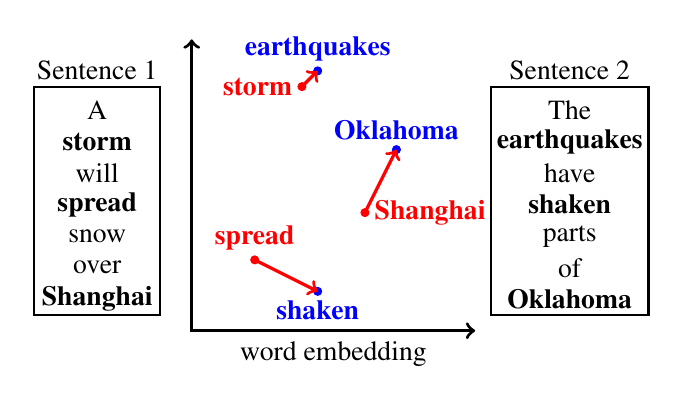
\begin{tikzpicture}
\draw [thick] (0.2, 0.5) rectangle (1.8, 3.4);
\draw [very thick, <->] (2.2, 4.0) -- (2.2, 0.3) -- (5.8, 0.3);
\draw [thick] (6.0, 0.5) rectangle (8.0, 3.4);

\node at (4.0, 0.0) {word embedding};

\node at (1.0, 3.6) {Sentence 1};
\node at (1.0, 3.1) {A};
\node at (1.0, 2.7) {\bf storm};
\node at (1.0, 2.3) {will};
\node at (1.0, 1.9) {\bf spread};
\node at (1.0, 1.5) {snow};
\node at (1.0, 1.1) {over};
\node at (1.0, 0.7) {\bf Shanghai};

\node at (7.0, 3.6) {Sentence 2};
\node at (7.0, 3.1) {The};
\node at (7.0, 2.7) {\bf earthquakes};
\node at (7.0, 2.3) {have};
\node at (7.0, 1.9) {\bf shaken};
\node at (7.0, 1.5) {parts};
\node at (7.0, 1.1) {of};
\node at (7.0, 0.7) {\bf Oklahoma};

\draw [fill, red] (3.6, 3.4) circle [radius=0.05];
\node [left, red] at (3.6, 3.4) {\bf storm};

\draw [fill, blue] (3.8, 3.6) circle [radius=0.05];
\node [above, blue] at (3.8, 3.6) {\bf earthquakes};

\draw [fill, red] (3.0, 1.2) circle [radius=0.05];
\node [above, red] at (3.0, 1.2) {\bf spread};

\draw [fill, blue] (3.8, 0.8) circle [radius=0.05];
\node [below, blue] at (3.8, 0.8) {\bf shaken};

\draw [fill, red] (4.4, 1.8) circle [radius=0.05];
\node [right, red] at (4.4, 1.8) {\bf Shanghai};

\draw [fill, blue] (4.8, 2.6) circle [radius=0.05];
\node [above, blue] at (4.8, 2.6) {\bf Oklahoma};

\draw [->, very thick, red] (3.6, 3.4) -- (3.8, 3.6);
\draw [->, very thick, red] (3.0, 1.2) -- (3.8, 0.8);
\draw [->, very thick, red] (4.4, 1.8) -- (4.8, 2.6);

\end{tikzpicture}
\caption{An illustration of the word mover's distance.}
\end{figure}
}
}


\frame{
{Word Embedding Feature Engineering}
\begin{block}{}
    \begin{columns}
        \column{0.1\textwidth}
        \column{0.4\textwidth}
                {\color{blue} Word Embedding}
                \begin{enumerate}
                \item word2vec
                \item GloVe
                \item C\&W
                \item Wiki
                \end{enumerate}
      \column{0.5\textwidth}
            {\color{blue} Distance Measurements}
            \begin{enumerate}
            \item Cosine Distance
            \item Manhattan Distance
            \item Euclidean Distance
            \item Pearson coefficient
            \item Spearman coefficient
            \item Kendall tau coefficient
            \end{enumerate}
    \end{columns}
\end{block}
}

\section{Experiments}


\subsection{Datasets and Evaluation}

\frame{
\frametitle{Datasets}
\begin{table}[h]
\tiny
\begin{center}
\begin{tabular}{crr|crr}
\hline
\hline
\multicolumn{3}{c|}{\bf{Training Set}} & \multicolumn{3}{c}{\bf{Test Set}} \\
\hline
\bf Dataset & \bf Input & \bf Gold  & \bf Dataset &  \bf Input & \bf Gold\\
\hline
\hline
MSRpar        & 1500    & 1500  & answers-answers   & 1572  & 254 \\
SMTeuroparl   & 1193    & 1193  & plagiarism        & 1271  & 230 \\
{\color{red}headlines*}    & 3000    & 2250  & {\color{red} headlines*}        & 1498  & 249 \\
SMTnews       & 399     &  399  & postediting       & 3287  & 244 \\
MSRvid        & 1500    & 1500  & question-question & 1555  & 209 \\
OnWN          & 2061    & 2061  & -&-&-  \\
FNWN          & 189     &  189  & -&-&-  \\
images        & 2250    &  1500 & -&-&-  \\
deft-forum    & 450     &  450  & -&-&-  \\
deft-news     & 300     &  300  & -&-&-  \\
tweet-news    & 750     &  750  & -&-&-  \\
answers-forums& 1500    &  375  & -&-&-  \\
answers-students&1500   &  750  & -&-&-  \\
belief        &2000     &  375  & -&-&-  \\
\hline
\hline
All           &19092    & 13592 & All  & 9183  & 1186 \\
\hline
\hline
\end{tabular}
\end{center}
\caption{The statistics of all datasets for STS task.}
\end{table}

}


\subsection{Questions}
\frame{
{Questions}
\begin{enumerate}
\item[$Q_1$] {\color{blue} {Supervised Model?}} \\
      {\color{red}  A: Learning Algorithm: SVM? RF? GB?}
      \vspace{0.2cm}
\item[$Q_2$] {\color{blue} Difference between Training Data and Test Data?} \\
      {\color{red} A: Training Data: All? Selected Data?}
       \vspace{0.2cm}
\item[$Q_3$] {\color{blue} Efficient Feature Set?} \\
      {\color{red} A: Feature Set: ? ? }
\end{enumerate}
}



%\subsection{Learning Algorithm}
\frame{
\frametitle{$Q_1:$ Learning Algorithm}

\begin{table}[h]
%\addtolength{\tabcolsep}{-2pt}
\tiny
\begin{center}
\begin{tabular}{c|ccccc|c}
\hline
\hline
\multirow{2}{*}{\bf Regression} & \multirow{2}{*}{\bf belief} & \bf answers & \multirow{2}{*}{\bf headlines} & \multirow{2}{*}{\bf images} & \bf answers & \bf Weighted \\
    & & \bf -students & & & \bf -forums & \bf Mean\\
\hline
\hline
\bf SVR(c=1) & 0.7413 &  0.7359  &  0.8168  &   0.8660  & 0.7400 & 0.7898 \\
\bf RF(n=40) & 0.7466 &  0.7100  &  0.8200  &   0.8534  & 0.7398 & 0.7816 \\
\bf GB(n=140)& \bf 0.7655 &   0.7484  &  \bf 0.8439  &   \bf 0.8791  & \bf 0.7469 & \bf 0.8080 \\
\hline
\hline
\bf DLSCU-S1 & 0.7491 &  \bf 0.7725  &  0.8250  &   0.8644  & 0.7390 & 0.8015 \\
\hline
\hline
\end{tabular}
\tiny{\caption{Results of different algorithm on STS 2015 test data.}} \label{tab:algorithmSelection}
\end{center}
\end{table}
}

\frame{
\frametitle{$Q_2:$ Training Data}

\begin{block}{Measurements}
    \begin{enumerate}
    \item source
    \item average length of sentences
    \item word mover's distance
    \end{enumerate}
\end{block}
%\cite{sultan-bethard-sumner:2015:SemEval} has shown that taking all the training datasets into consideration may hurt the performance since training and test sets are from different domains. Hence, for each test set, we select the datasets which are most similar, taking source, average length of sentences and word mover's distance(discussed in Section \ref{ssec:word embedding feature engineering}) into consideration.
\begin{block}{Training Data for STS 2016 test data}
    \begin{enumerate}
    \item \textbf{headlines}: {\color{red}headlines}
    \item \textbf{answers-answers, question-question}:  \\
            {\color{red}belief, deft-forums, answers-students, answers-forums}
    \item \textbf{postediting}: {\color{red}SMTeuropar, MSRpar}
    \item \textbf{plagiarism}: {\color{red}onWN, FNWN}
    %For the data set with symbol * (i.e., {\em headlines}), we use all {\em headlines} pairs.  For {\em answers-answers} and {\em question-question}, we use {\em belief, deft-forums, answers-students, answers-forums} pairs. For postediting, we use {\em SMTeuropar} and {\em MSRpar} pairs. For plagiarism, we use {\em onWN} and {\em FNWN} pairs.
    \end{enumerate}
\end{block}
}


\frame{
\frametitle{$Q_3:$ Feature Selection}
\begin{table}[h]
\addtolength{\tabcolsep}{-3pt}
\tiny
\begin{center}
\begin{tabular}{cl|c|c|c|c|c}
\hline
\hline
\multicolumn{2}{c|}{\multirow{2}{*}{\bf Feature}} & \bf \multirow{2}{*}{belief} & \bf answers & \bf \multirow{2}{*}{headlines} & \bf \multirow{2}{*}{image} & \bf answers \\
   &    &   & \bf -students &   &   & \bf-forums \\
\hline
\hline
\multirow{5}{*}{\bf String-based}   & len   &     -   &  -      & $\surd$ & $\surd$ &  -        \\
                                    & pos   &     -   &  -      & $\surd$ & -       & $\surd$   \\
                                    & lcs   &     -   &  -      & $\surd$ & $\surd$ & $\surd$   \\
                                    & ngram &     -   & $\surd$ & $\surd$ & $\surd$ & $\surd$   \\
                                    & ner   &     -   & $\surd$ & $\surd$ &  -      &  -         \\
\hline
\multirow{2}{*}{ \tabincell{c}{\bf Machine\\ \bf Translation}}
                                    & average& $\surd$&  -      & $\surd$ & $\surd$ &  -        \\
                                    & \color{red} concat&   \color{red}   -   & \color{red}  -      &  \color{red} -      &  \color{red}   -    & \color{red}  -        \\
\hline
\multirow{2}{*}{\bf Corpus-based}   &wordnet&$\surd$  & $\surd$ & $\surd$ &  -      & $\surd$   \\
                                    & lsa   &     -   & $\surd$ & $\surd$ & $\surd$ & $\surd$   \\
\hline
\multirow{2}{*}{\bf Alignment}      & global&     -   & $\surd$ & $\surd$ & $\surd$ & $\surd$   \\
                                    & specific&$\surd$& $\surd$ & $\surd$ & $\surd$ & $\surd$   \\
\hline
\hline
\multirow{3}{*}{ \tabincell{c}{\bf Word Centroid \\ \bf Distance} }\
                                    & word2vec&$\surd$& $\surd$ & $\surd$ & $\surd$ & $\surd$   \\
                                    & \color{red} glove   &  \color{red}  -   & \color{red}    -    & \color{red}  -      & \color{red} -       &  \color{red} -        \\
                                    & turian's&$\surd$& $\surd$ & $\surd$ & $\surd$ &  -        \\
\hline
\tabincell{c}{\bf Word Mover's \\ \bf Distance}
                                    & wmd     &$\surd$& $\surd$ & $\surd$ & $\surd$ & $\surd$   \\
\hline
\hline
\multicolumn{2}{c|}{\bf Our Results} & \bf 0.7835 & 0.7713 & \bf 0.8455 & \bf 0.8808 & \bf 0.7636 \\
\hline
\multicolumn{2}{c|}{\bf Best Scores}  & 0.7717 & \bf 0.7879 & 0.8417 & 0.8713 & 0.7390 \\
\hline
\hline
\end{tabular}
\end{center}
\caption{Results of feature selection experiments on STS 2015 test data.}
 %The last row shows the the best scores of all submitted system on STS 2015 task.
\label{tab:train}
\end{table}
}

\subsection{Setups}
\frame{
{Setups}

\begin{itemize}
\item U-SEVEN:
    \begin{enumerate}
        \item longest common sequence
        \item alignment feature
        \item corpus-based feature
        \item word centroid distance from from four word embedding.\\
             cosine distance, Pearson coefficient, Spearman coefficient.
    \end{enumerate}
\item S1-All
     \begin{enumerate}
        \item all the training datasets
        \item regression model: GB(n=140)
        \item feature selection: hill climbing
    \end{enumerate}
\item S2
    \begin{enumerate}
        \item selected training datasets
        \item regression model: GB(n=140)
        \item feature selection: hill climbing
    \end{enumerate}
\end{itemize}
}


\section{Results on Test Data}

\frame{
\frametitle{Results}
\begin{table}[h]
\footnotesize
\begin{center}
\begin{tabular}{c|ccc|c}
\hline
\hline
\multirow{2}{*}{\bf Dataset} & \multicolumn{3}{c|}{\bf Runs}  & \bf Best \\
                              \cline{2-4}
                              & \bf U-SEVEN & \bf S1-All & \bf S2 & \bf Score \\
\hline
\hline
\bf answers-answers &     0.4774  &     0.5697 & \bf 0.5715 & 0.6923\\
\bf plagiarism      & \bf 0.8301  &     0.8250 &     0.7733 & 0.8413\\
\bf headlines       &     0.7668  & \bf 0.8121 &     0.7903 & 0.8274\\
\bf postediting     & \bf 0.8423  &     0.8234 &     0.7496 & 0.8669\\
\bf question-question&    0.7191  & \bf 0.7311 &     0.6763 & 0.7470\\
\hline
\hline
\bf weighted mean   &     0.7242  & \bf 0.7507 &     0.7116 & 0.7780\\
\hline
\hline
\end{tabular}
\end{center}
\caption{The results of our three runs on STS 2016 test datasets.}\label{tab:test}
\end{table}
}


\frame{
\frametitle{Results}
$
\left\{ \begin{array}{ll}
\textrm{ You should do it.}\\
\textrm{ You can do it, too.} \\
\end{array} \color{red}{ \qquad \  \text{\quad \ (sys: 4.0 / gs: 1.0)}} \right.
$
$
\left\{ \begin{array}{ll}
\textrm{ It's pretty much up to you.}\\
\textrm{ It's much better to ask.} \\
\end{array} \color{red}{ \text{ (sys: 3.2 / gs: 0.0)}} \right.
$
}

\section{Conclusion}

\frame{
{Conclusion}
\begin{enumerate}
\item The difference between top system and our best system is about 2.8\%
\item Future work: Deep Learning
\end{enumerate}
}

\end{document}
